\section{Improper Integrals} \label{S:5.5.Improper}

\begin{goals}
  \item What are improper integrals and why are they important?
  \item What does it mean to say that an improper integral converges or diverges?
  \item What are some typical improper integrals that we can classify as convergent or divergent? 
\end{goals}

%--------------------------------------
% SUBSECTION INTRODUCTION
%--------------------------------------
\subsection*{Introduction}

Another important application of the definite integral 
regards how the likelihood of certain events can be measured.  For example, consider a company that manufactures incandescent light bulbs, and suppose that based on a large volume of test results, they have determined that the fraction of light bulbs that fail between times $t = a$ and $t = b$ of use (where $t$ is measured in months) is given by 
$$\int_a^b 0.3 e^{-0.3t} \, dt.$$
For example, the fraction of light bulbs that fail during their third month of use is given by
\begin{eqnarray*} 
\int_2^3 0.3e^{-0.3t} \, dt & = & -e^{-0.3t} \bigg \vert_2^3 \\
				& = & -e^{-0.9} + e^{-0.6} \\
				& \approx & 0.1422.
\end{eqnarray*}
Thus about 14.22\% of all lightbulbs fail between $t = 2$ and $t = 3$.  %In our upcoming study of the concept of \emph{probability} in Section~\ref{S:6.6.Prob}, we'll also see how such an integral represents the likelihood that a randomly chosen light bulb fails between $t = 2$ and $t = 3$.  
Clearly we could adjust the limits of integration to measure the fraction of light bulbs that fail during any time period of interest.

\begin{pa} \label{PA:5.5}  A company with a large customer base has a call center that receives thousands of calls a day.  After studying the data that represents how long callers wait for assistance, they find that the function $p(t) = 0.25e^{-0.25t}$ models the time customers wait in the following way:  the fraction of customers who wait between $t = a$ and $t = b$ minutes is given by
$$\int_a^b p(t) \, dt.$$  
Use this information to answer the following questions.
\ba
	\item Determine the fraction of callers who wait between $5$ and $10$ minutes.
	\item Determine the fraction of callers who wait between $10$ and $20$ minutes.
	\item Next, let's study how the fraction who wait up to a certain number of minutes:
	\begin{itemize}
		\item[i.] What is the fraction of callers who wait between $0$ and $5$ minutes?
		\item[ii.] What is the fraction of callers who wait between $0$ and $10$ minutes?
		\item[iii.] Between $0$ and $15$ minutes?  Between $0$ and $20$? 
	\end{itemize}
	\item Let $F(b)$ represent the fraction of callers who wait between $0$ and $b$ minutes.  Find a formula for $F(b)$ that involves a definite integral, and then use the First FTC to find a formula for $F(b)$ that does not involve a definite integral.
	\item What is the value of $\ds \lim_{b \to \infty} F(b)$?  Why?
\ea
\end{pa} 
\afterpa % PREVIEW ACTIVITY

%--------------------------------------------------------------
% SUBSECTION IMPROPER INTEGRALS INVOLVING UNBOUNDED INTERVALS
%--------------------------------------------------------------
\subsection*{Improper Integrals Involving Unbounded Intervals} \index{improper integral}

In light of our example with light bulbs that fail, as well as with the problem involving customer wait time in Preview Activity~\ref{PA:5.5}, we see that it is natural to consider questions where we desire to integrate over an interval whose upper limit grows without bound.  For example, if we are interested in the fraction of light bulbs that fail within the first $b$ months of use, we know that the expression
$$\int_0^b 0.3e^{-0.3t} \, dt$$
measures this value.  To think about the fraction of light bulbs that fail \emph{eventually}, we understand that we wish to find
$$\lim_{b \to \infty} \int_0^b 0.3e^{-0.3t} \, dt,$$
for which we will also use the notation 
\begin{equation} \label{E:ImpInt1}
\int_0^\infty 0.3e^{-0.3t} \, dt.
\end{equation}
Note particularly that we are studying the area of an unbounded region, as pictured in Figure~\ref{F:5.5.InfReg}.

\begin{marginfigure} % MARGIN FIGURE
%\begin{center}
\margingraphics{figures/6_5_InfReg.eps}
\caption{At left, the area bounded by $p(t) = 0.3e^{-0.3t}$ on the finite interval $[0,b]$; at right, the result of letting $b \to \infty$.  By ``$\cdots$'' in the righthand figure, we mean that the region extends to the right without bound.} \label{F:5.5.InfReg}
%\end{center}
\end{marginfigure}

Anytime we are interested in an integral for which the interval of integration is unbounded (that is, one for which at least one of the limits of integration involves $\infty$), we say that the integral is {\bf improper}\index{improper integral!unbounded region of integration}.  For instance, the integrals
$$\int_1^{\infty} \frac{1}{x^2} \, dx, \ \ \int_{-\infty}^0 \frac{1}{1+x^2} \, dx, \ \ \mbox{and} \int_{-\infty}^{\infty} e^{-x^2} \, dx$$
are all improper due to having limits of integration that involve $\infty$.  We investigate the value of any such integral be replacing the improper integral with a limit of proper integrals; for an improper integral such as $\int_0^\infty f(x) \, dx$, we write
$$\int_0^\infty f(x) \, dx = \lim_{b \to \infty} \int_0^b f(x) \,dx.$$
We can then attempt to evaluate $\int_0^b f(x) \,dx$ using the FTC, after which we can evaluate the limit.  An immediate and important question arises: is it even possible for the area of such an unbounded region to be finite?  The following activity explores this issue and others in more detail.

\begin{activity} \label{A:5.5.1}  In this activity we explore the improper integrals $\ds \int_1^{\infty} \frac{1}{x} \, dx$ and $\ds \int_1^{\infty} \frac{1}{x^{3/2}} \, dx$.
\ba
	\item First we investigate $\ds \int_1^{\infty} \frac{1}{x} \, dx$.
	\be
		\item[i.] Use the First FTC to determine the exact values of $\ds \int_1^{10} \frac{1}{x} \, dx$, $\ds \int_1^{1000} \frac{1}{x} \, dx$, and $\ds \int_1^{100000} \frac{1}{x} \, dx$.  Then, use your calculator to compute a decimal approximation of each result.
		\item[ii.]  Use the First FTC to evaluate the definite integral $\ds \int_1^{b} \frac{1}{x} \, dx$ (which results in an expression that depends on $b$).
		\item[iii.]  Now, use your work from (ii.) to evaluate the limit given by
	$$\lim_{b \to \infty}  \int_1^{b} \frac{1}{x} \, dx.$$
	\ee
	\item Next, we investigate $\ds \int_1^{\infty} \frac{1}{x^{3/2}} \, dx$.
	\be
		\item[i.] Use the First FTC to determine the exact values of $\ds \int_1^{10} \frac{1}{x^{3/2}} \, dx$, $\ds \int_1^{1000} \frac{1}{x^{3/2}} \, dx$, and $\ds \int_1^{100000} \frac{1}{x^{3/2}} \, dx$.  Then, use your calculator to compute a decimal approximation of each result.
		\item[ii.]  Use the First FTC to evaluate the definite integral $\ds \int_1^{b} \frac{1}{x^{3/2}} \, dx$ (which results in an expression that depends on $b$).
		\item[iii.]  Now, use your work from (ii.) to evaluate the limit given by
	$$\lim_{b \to \infty}  \int_1^{b} \frac{1}{x^{3/2}} \, dx.$$
	\ee
	\item Plot the functions $y = \frac{1}{x}$ and $y = \frac{1}{x^{3/2}}$ on the same coordinate axes for the values $x = 0 \ldots 10$.  How would you compare their behavior as $x$ increases without bound?  What is similar?  What is different?
	\item How would you characterize the value of $\ds \int_1^{\infty} \frac{1}{x} \, dx$? of $\ds \int_1^{\infty} \frac{1}{x^{3/2}} \, dx$?  What does this tell us about the respective areas bounded by these two curves for $x \ge 1$?
\ea

\end{activity}
\begin{smallhint}
\ba
	\item Small hints for each of the prompts above.
\ea
\end{smallhint}
\begin{bighint}
\ba
	\item Big hints for each of the prompts above.
\ea
\end{bighint}
\begin{activitySolution}
\ba
	\item Solutions for each of the prompts above.
\ea
\end{activitySolution}
\aftera %ACTIVITY

\begin{example} \label{eg:5.5.1} % EXAMPLE
Evaluate the following improper integrals.

\bmtwo
\begin{enumerate}[1)]
\item		$\ds\int_1^\infty \frac1{x^2}\ dx$
\item		$\ds\int_1^\infty \frac1{\sqrt{x}}\ dx$
\item		$\ds\int_{-\infty}^0 e^x\ dx$
\item		$\ds\int_{-\infty}^\infty \frac1{1+x^2}\ dx$
\end{enumerate}
\emtwo


\solution
\begin{enumerate}[1)]
\item	$\begin{aligned}[t] 
\int_1^\infty \frac{1}{x^2}\ dx &= \lim_{b\to\infty} \int_1^b\frac1{x^2}\ dx \\ 
&= \lim_{b\to\infty} \frac{-1}{x}\Big|_1^b \\
&= \lim_{b\to\infty} \frac{-1}{b} + 1\\
&= 1.
\end{aligned}$

A graph of the area defined by this integral is given in Figure~\ref{F:5-5-EG1}-(a).
 
\item $\begin{aligned}[t]
\int_1^\infty \frac1{\sqrt{x}}\ dx & = \lim_{b\to\infty}\int_1^b\frac1{\sqrt{x}}\ dx \\
&= \lim_{b\to\infty} 2\sqrt{x}\Big|_1^b \\
&= \lim_{b\to\infty} 2\sqrt{b}-2 \\
&= \infty.
\end{aligned}$
	
The limit does not exist, hence the improper integral $\ds\int_1^\infty\frac1x\ dx$ does not exist. %Compare the graphs in Figures \ref{fig:impint1a} and \ref{fig:impint1b}; notice how the graph of $f(x) = 1/x$ is noticeably larger. This difference is enough to cause the improper integral to diverge.

\item $\begin{aligned}[t]
\int_{-\infty}^0 e^x \ dx &= \lim_{a\to-\infty} \int_a^0e^x\ dx \\
&=  \lim_{a\to-\infty} e^x\Big|_a^0 \\
&= \lim_{a\to-\infty} e^0-e^a \\
&= 1.
\end{aligned}$
		
A graph of the area defined by this integral is given in Figure~\ref{F:5-5-EG1}-(c).

\item We will need to break this into two improper integrals and choose a value of $c \in (-\infty,\infty)$. Any value of $c$ is fine; we choose $c=0$.
\begin{align*}%
\int_{-\infty}^\infty \frac1{1+x^2}\ dx &= \lim_{a\to-\infty} \int_a^0\frac{1}{1+x^2}\ dx + \lim_{b\to\infty} \int_0^b\frac{1}{1+x^2}\ dx \\
&= \lim_{a\to-\infty} \arctan(x)\Big|_a^0 + \lim_{b\to\infty} \arctan(x)\Big|_0^b\\
\intertext{\[= \lim_{a\to-\infty} \left(\arctan(0)-\arctan(a)\right) + \lim_{b\to\infty} \left(\arctan(b)-\arctan(0)\right)\]}
&= \left(0-\frac{-\pi}2\right) + \left(\frac{\pi}2-0\right).\\
\intertext{Each	limit exists, hence the original integral converges and has value:}
&= \pi.
\end{align*}

A graph of the area defined by this integral is given in Figure~\ref{F:5-5-EG1}-(d).
\end{enumerate}
\end{example}

\begin{marginfigure}
\begin{center}
\subfloat[A graph of $f(x) = \frac{1}{x^2}$.]{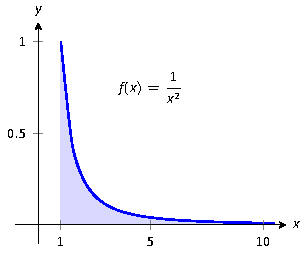
\includegraphics[scale=.75]{figures/figeximpint1a} }

\subfloat[A graph of $f(x) = \frac{1}{\sqrt{x}}$.]{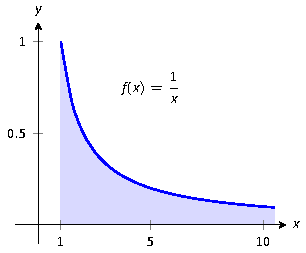
\includegraphics[scale=.75]{figures/figeximpint1b}}

\subfloat[A graph of $f(x) = e^x$.]{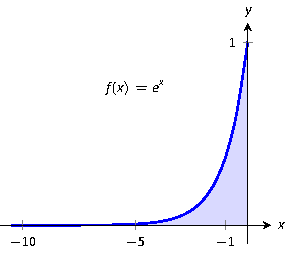
\includegraphics[scale=.75]{figures/figeximpint1c}}

\subfloat[A graph of $f(x) = \frac{1}{1+x^2}$.]{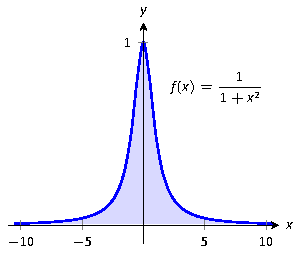
\includegraphics[scale=.75]{figures/figeximpint1d}}
\caption{The various graphs used  in Example~\ref{eg:5.5.1}.}
\label{F:5-5-EG1}
\end{center}
\end{marginfigure} %EXAMPLE

%--------------------------------------------------------------
% SUBSECTION CONVERGENCE AND DIVERGENCE
%--------------------------------------------------------------
\subsection*{Convergence and Divergence} 

Our work so far has suggested that when we consider a nonnegative function $f$ on an interval $[1,\infty]$, such as $f(x) = \frac{1}{x}$ or $f(x) = \frac{1}{x^{3/2}}$, there are at least two possibilities for the value of $\lim_{b \to \infty} \int_1^b f(x) \, dx$:  the limit is finite or infinite.  With these possibilities in mind, we introduce the following terminology.

\concept{Convergence of Improper Integrals with Infinite Bounds} %CONCEPT
{If $f(x)$ is nonnegative for $x \ge a$, then we say that the improper integral $\int_a^{\infty} f(x) \, dx$
\emph{converges}\index{improper integral!converges} provided that 
$$\lim_{b \to \infty} \int_a^{b} f(x) \, dx$$
exists and is finite.  Otherwise, we say that $\int_a^{\infty} f(x) \, dx$ \emph{diverges}\index{improper integral!diverges}.
} %end CONCEPT

We normally restrict our interest to improper integrals for which the integrand is nonnegative.  Further, we note that our primary interest is in functions $f$ for which $\lim_{x \to \infty} f(x) = 0$, for if the function $f$ does not approach $0$ as $x \to \infty$, then it is impossible for $\int_a^{\infty} f(x) \, dx$ to converge.

\begin{activity} \label{A:5.5.2}  Determine whether each of the following improper integrals converges or diverges.  For each integral that converges, find its exact value.
\ba
	\item $\ds \int_1^{\infty} \frac{1}{x^2} \, dx$
	\item $\ds \int_0^{\infty} e^{-x/4} \, dx$
	\item $\ds \int_2^{\infty} \frac{9}{(x+5)^{2/3}} \, dx$
	\item $\ds \int_4^{\infty} \frac{3}{(x+2)^{5/4}} \, dx$
	\item $\ds \int_0^{\infty} x e^{-x/4} \, dx$ 
	%\item $\ds \int_1^{\infty} \frac{1}{x^p} \, dx$, where $p$ is a positive real number
\ea

\end{activity}
\begin{smallhint}
\ba
	\item Small hints for each of the prompts above.
\ea
\end{smallhint}
\begin{bighint}
\ba
	\item Big hints for each of the prompts above.
\ea
\end{bighint}
\begin{activitySolution}
\ba
	\item Solutions for each of the prompts above.
\ea
\end{activitySolution}
\aftera %ACTIVITY

\begin{marginfigure}[4CM]
\margingraphics{figures/figeximpint2} %EXAMPLE 192 APEX
\caption{A graph of $f(x) = \frac{\ln(x)}{x^2}$ in Example \ref{eg:5.5.2}}
\label{F:5-5_Eg2}
\end{marginfigure}

\begin{example} \label{eg:5.5.2} % EXAMPLE
Evaluate the improper integral $\ds \int_1^\infty \frac{\ln( x)}{x^2}\ dx.$

\solution This integral will require the use of Integration by Parts. Let $u = \ln (x)$ and $dv = 1/x^2\ dx$. Then
\begin{align*}
\int_1^\infty\frac{\ln (x)}{x^2}\ dx &= \lim_{b\to\infty}\int_1^b\frac{\ln (x)}{x^2}\ dx \\
&=  \lim_{b\to\infty}\left(-\frac{\ln (x)}{x}\Big|_1^b +\int_1^b \frac{1}{x^2} \ dx \right)\\
&=  \lim_{b\to\infty} \left.\left(-\frac{\ln (x)}{x} -\frac1x\right)\right|_1^b\\
&=	\lim_{b\to\infty} \left(-\frac{\ln (b)}{b}-\frac1b - \left(-\ln (1)-1\right)\right).\\
\intertext{The $1/b$ and $\ln (1)$ terms go to $0$, leaving $\ds \lim_{b\to\infty} -\frac{\ln (b)}b + 1.$ We need to evaluate $\ds \lim_{b\to\infty} \frac{\ln (b)}{b}$ with l'H\^opital's Rule. We have:}
\lim_{b\to\infty}\frac{\ln (b)}b &\stackrel{\ \text{ by LHR \rule[-5pt]{0pt}{3pt}} \ }{=} \lim_{b\to\infty} \frac{1/b}{1} \\
&= 0.
\intertext{Thus the improper integral evaluates as: }
\int_1^\infty\frac{\ln (x)}{x^2}\ dx &= 1.
\end{align*}

\end{example} %EXAMPLE

%--------------------------------------------------------------
% SUBSECTION IMPROPER INTEGRALS INVOLVING UNBOUNDED INTEGRANDS
%--------------------------------------------------------------
\subsection*{Improper Integrals Involving Unbounded Integrands}

It is also possible for an integral to be improper due to the integrand being unbounded on the interval of integration.  For example, if we consider 
$$\int_0^1 \frac{1}{\sqrt{x}} \, dx,$$
we see that because $f(x) = \frac{1}{\sqrt{x}}$ has a vertical asymptote at $x = 0$, $f$ is not continuous on $[0,1]$, and the integral is attempting to represent the area of the unbounded region shown at right in Figure~\ref{F:5.5.InfIntegrand}.

\begin{marginfigure}[-1cm] % MARGIN FIGURE
\margingraphics{figures/6_5_InfIntegrand.eps}
\caption{At left, the area bounded by $f(x) = \frac{1}{\sqrt{x}}$ on the finite interval $[a,1]$; at right, the result of letting $a \to 0^+$, where we see that the shaded region will extend vertically without bound.} \label{F:5.5.InfIntegrand}
\end{marginfigure}

Just as we did with improper integrals involving infinite limits, we address the problem of the integrand being unbounded\index{improper integral!unbounded integrand} by replacing such an improper integral with a limit of proper integrals.  For example, to evaluate $\int_0^1 \frac{1}{\sqrt{x}} \, dx$, we replace $0$ with $a$ and let $a$ approach $0$ from the right.  Thus,
$$\int_0^1 \frac{1}{\sqrt{x}} \, dx = \lim_{a \to 0^+} \int_a^1 \frac{1}{\sqrt{x}} \, dx,$$
and then we evaluate the proper integral $\int_a^1 \frac{1}{\sqrt{x}} \, dx$, followed by taking the limit.  In the same way as with improper integrals involving unbounded regions, we will say that the improper integral converges provided that this limit exists, and diverges otherwise.  In the present example, we observe that
\begin{eqnarray*}
\int_0^1 \frac{1}{\sqrt{x}} \, dx & = & \lim_{a \to 0^+} \int_a^1 \frac{1}{\sqrt{x}} \, dx \\
					& = & \lim_{a \to 0^+} 2\sqrt{x} \big\vert_a^1 \\
					& = & \lim_{a \to 0^+} 2\sqrt{1} - 2\sqrt{a} \\
					& = & 2,
\end{eqnarray*}
and therefore the improper integral $\int_0^1 \frac{1}{\sqrt{x}} \, dx$ converges (to the value $2$).

We have to be particularly careful with unbounded integrands, for they may arise in ways that may not initially be obvious.  Consider, for instance, the integral
$$\int_1^3 \frac{1}{(x-2)^2} \, dx.$$
At first glance we might think that we can simply apply the Fundamental Theorem of Calculus by antidifferentiating $\frac{1}{(x-2)^2}$ to get $-\frac{1}{x-2}$ and then evaluate from $1$ to $3$.  Were we to do so, we would be erroneously applying the FTC because $f(x) = \frac{1}{(x-2)^2}$ fails to be continuous throughout the interval, as seen in Figure~\ref{F:5.5.InfIntegrand2}.

\begin{marginfigure} % MARGIN FIGURE
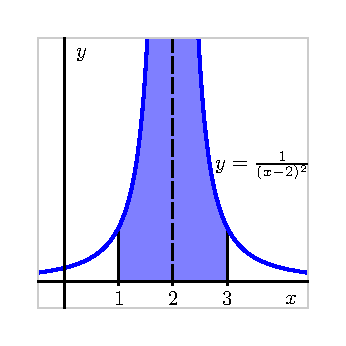
\includegraphics{figures/6_5_InfIntegrand2.eps}
\caption{The function $f(x) = \frac{1}{(x-2)^2}$ on an interval including $x = 2$.} \label{F:5.5.InfIntegrand2}
\end{marginfigure}

Such an incorrect application of the FTC leads to an impossible result ($-2$), which would itself suggest that something we did must be wrong.  Indeed, we must address the vertical asymptote in $f(x) = \frac{1}{(x-2)^2}$ at $x = 2$ by writing
$$\int_1^3 \frac{1}{(x-2)^2} \, dx = \lim_{a \to 2^-} \int_1^a \frac{1}{(x-2)^2} \, dx + \lim_{b \to 2^+} \int_b^3 \frac{1}{(x-2)^2} \, dx$$
and then evaluate two separate limits of proper integrals.  For instance, doing so for the integral with $a$ approaching $2$ from the left, we find 
\begin{eqnarray*}
\int_1^2 \frac{1}{(x-2)^2} \, dx & = & \lim_{a \to 2^-} \int_1^a \frac{1}{(x-2)^2} \, dx \\
						& = & \lim_{a \to 2^-} -\frac{1}{(x-2)} \bigg\vert_1^a \\
						& = & \lim_{a \to 2^-} -\frac{1}{(a-2)} + \frac{1}{1-2} \\
						& = & \infty,
\end{eqnarray*}
since $\frac{1}{a-2} \to -\infty$ as $a$ approaches $2$ from the left.  Thus, the improper integral $\int_1^2 \frac{1}{(x-2)^2} \, dx$ diverges; similar work shows that $\int_2^3 \frac{1}{(x-2)^2} \, dx$ also diverges.  From either of these two results, we can conclude that  that the original integral, $\int_1^3 \frac{1}{(x-2)^2} \, dx$ diverges, too.  

\begin{activity} \label{A:5.5.3}  For each of the following definite integrals, decide whether the integral is improper or not.  If the integral is proper, evaluate it using the First FTC.  If the integral is improper, determine whether or not the integral converges or diverges; if the integral converges, find its exact value. 
\bmtwo
\ba
	\item $\ds \int_0^1 \frac{1}{x^{1/3}} \, dx$
	\item $\ds \int_0^2 e^{-x} \, dx$
	\item $\ds \int_1^4 \frac{1}{\sqrt{4-x}} \, dx$
	\item $\ds \int_{-2}^2 \frac{1}{x^2} \, dx$
	\item $\ds \int_0^{\pi/2} \tan(x) \, dx$
	\item $\ds \int_0^1 \frac{1}{\sqrt{1-x^2}} \, dx$
\ea
\emtwo

\end{activity}
\begin{smallhint}
\ba
	\item Small hints for each of the prompts above.
\ea
\end{smallhint}
\begin{bighint}
\ba
	\item Big hints for each of the prompts above.
\ea
\end{bighint}
\begin{activitySolution}
\ba
	\item Solutions for each of the prompts above.
\ea
\end{activitySolution}
\aftera %ACTIVITY

\begin{marginfigure}[8cm]
\margingraphics{figures/figimpint3b} %EXAMPLE 193b APEX
\caption{A graph of $f(x)=\frac{1}{x^2}$ in Example~\ref{eg:5.5.3}}
\label{F:5-5_Eg3}
\end{marginfigure}

\begin{example} \label{eg:5.5.3} % EXAMPLE
Evaluate the following improper integral: $\ds  \int_{-1}^1\frac{1}{x^2}\ dx.$

\solution The function $f(x) = 1/x^2$ has a vertical asymptote at $x=0$, as shown in Figure \ref{F:5-5_Eg3}, so this integral is an improper integral. Let's eschew using limits for a moment and proceed without recognizing the improper nature of the integral. This leads to:
\begin{align*}
\int_{-1}^1\frac1{x^2}\ dx &= -\frac1x\Big|_{-1}^1\\
&= -1 - (1)\\
&=-2 
\end{align*}

Clearly the area in question is above the $x$-axis, yet the area is supposedly negative! Why does our answer not match our intuition?  Because the function has a vertical asymptote at $x = 0$. To answer this, evaluate 
\begin{align*}
\int_{-1}^1\frac1{x^2}\ dx &= \lim_{t\to0^-}\int_{-1}^t \frac1{x^2}\ dx + \lim_{t\to0^+}\int_t^1\frac1{x^2}\ dx \\
&= \lim_{t\to0^-}-\frac1x\Big|_{-1}^t + \lim_{t\to0^+}-\frac1x\Big|_t^1\\
&= \lim_{t\to0^-}-\frac1t-1 + \lim_{t\to0^+} -1+\frac1t\\
&\Rightarrow \Big(\infty-1\Big)\ + \ \Big(- 1+\infty\Big).
\end{align*}
Neither limit converges hence the original improper integral diverges. The nonsensical answer we obtained by ignoring the improper nature of the integral is just that: nonsensical.

\end{example} %EXAMPLE

%--------------------------------------------------------------
% SUBSECTION MORE ON CONVERGENCE AND DIVERGENCE
%--------------------------------------------------------------
\subsection*{More on Convergence and Divergence} 

Oftentimes we are interested in knowing simply whether or not an improper integral converges, and not necessarily the value of a convergent integral. There are many integrands that do not have an antiderivative expressible in terms of elementary functions, e.g., $\int_1^{\infty} e^{-x^2} \, dx$. We examine some tools for determining whether such an integral converges or diverges. 
A basic technique in determining convergence of improper integrals is to compare an integrand whose convergence is unknown to an integrand whose convergence is known. We often use integrands of the form $1/x\hskip1pt ^p$ to compare to as their convergence on certain intervals is known. The following activity explores for what values of $p$ do improper integrals involving $1/x\hskip1pt ^p$ converge. 

\begin{activity} \label{A:5.5.4}  The goal of this activity is understand the behavior of improper integrals involving $1/x^p$ for different values of $p$. 

\noindent 1)  Determine the values of $p$ for which $\ds \int_1^{\infty} \frac{1}{x^p} \, dx$ converges using the steps below.

\ba
\item Use the techniques discussed in this section to express  $\ds \int_1^{\infty} \frac{1}{x^p} \, dx$ as a limit. The limit should depend on $p$.
\item If $p>1$, does the limit exist? If it exists find its value.
\item If $p<1$, does the limit exist? If it exists find its value.
\item For what values of $p$, does $\ds \int_1^{\infty} \frac{1}{x^p} \, dx$ converge?
\item For what values of $p$, does $\ds \int_1^{\infty} \frac{1}{x^p} \, dx$ diverge?
\ea

\noindent 2) Determine the values of $p$ for which $\ds \int_0^1 \frac{1}{x^p} \, dx$ converges using the steps below.
\ba
\item Use the techniques discussed in this section to express  $\ds \int_0^1 \frac{1}{x^p} \, dx$ as a limit. The limit should depend on $p$.
\item If $p>1$, does the limit exist? If it exists find its value.
\item If $p<1$, does the limit exist? If it exists find its value.
\item For what values of $p$, does $\ds \int_0^1 \frac{1}{x^p} \, dx$ converge?
\item For what values of $p$, does $\ds \int_0^1 \frac{1}{x^p} \, dx$ diverge?
\ea


\end{activity}
\begin{smallhint}
\ba
	\item Small hints for each of the prompts above.
\ea
\end{smallhint}
\begin{bighint}
\ba
	\item Big hints for each of the prompts above.
\ea
\end{bighint}
\begin{activitySolution}
\ba
	\item Solutions for each of the prompts above.
\ea
\end{activitySolution}
\aftera %ACTIVITY   for integrals involving 1/x^p

Let's see how we can use the results of Activity \ref{A:5.5.4} to determine whether the integral $\int_1^{\infty} e^{-x^2} \, dx$ converges or diverges. First we compare the graphs of $f(x) = e^{-x^2}$ and $g(x)=1/x^2$. In Figure \ref{F:5.5.impint5}, we see that for $x\geq 1$, $0< f(x) < g(x)$.  We also have that the area under $f(x)$ is less than the area under $g(x)$, that is 
$$0 \leq \int_1^{\infty} e^{-x^2} \, dx \leq \int_1^{\infty} \frac1{x^2} \, dx.$$
We can then use the results of Activity \ref{A:5.5.4} (here $p=2$) or Example~\ref{eg:5.5.1} to get 
$$ 0 \leq \int_1^{\infty} e^{-x^2} \, dx \leq 1.$$

\begin{marginfigure} % MARGIN FIGURE
\margingraphics{figs/5/improperfg.pdf}
\caption{Graphs of $f(x) = e^{-x^2}$ and $f(x)= 1/x^2$.}
\label{F:5.5.impint5}
\end{marginfigure}

Therefore the integral $\int_1^{\infty} e^{-x^2} \, dx$ converges since its value is bounded by finite values. This technique to determine convergence is generalized in the following concept. 

\concept{Direct Comparison Test for Improper Integrals}  %CONCEPT
{Let $f$ and $g$ be continuous on $[a,\infty)$ where $0\leq f(x)\leq g(x)$ for all $x$ in $[a,\infty)$. 
	\begin{enumerate}[1)]
	\item		If $\ds \int_a^\infty g(x)\ dx$ converges, then $\ds \int_a^\infty f(x)\ dx$ converges.
	\index{integration!improper}\index{convergence!Direct Comparison Test!for integration}\index{divergence!Direct Comparison Test!for integration}\index{Direct Comparison Test!for integration}\index{convergence!of improper int.}\index{divergence!of improper int.}
	\item		If $\ds \int_a^\infty f(x)\ dx$ diverges, then $\ds \int_a^\infty g(x)\ dx$ diverges.
	\end{enumerate}
} %end CONCEPT

\begin{marginfigure}[4cm]
\margingraphics{figs/5/improperfgb} %EXAMPLE 195b APEX
\caption{A graph of $f(x)=\frac{1}{\sqrt{x^2-x}}$ and $g(x)= \frac{1}{x}$ in Example \ref{eg:5.5.4}}
\label{F:5-5_Eg4}
\end{marginfigure}

\begin{example} \label{eg:5.5.4} % EXAMPLE
Determine the convergence of the following improper integral:
$\ds  \int_{-1}^1\frac{1}{\sqrt{x^2-x}}\ dx.$

\solution
Note that for large values of $x$, $\ds \frac{1}{\sqrt{x^2-x}} \approx \frac{1}{\sqrt{x^2}} =\frac{1}{x}$. We know from Activity \ref{A:5.5.4} that  $\ds \int_3^\infty \frac1x\ dx$ diverges, so we seek to compare the original integrand to $1/x$.

It is easy to see that when $x>0$, we have $x = \sqrt{x^2} > \sqrt{x^2-x}$. Taking reciprocals reverses the inequality, giving $$\frac1x < \frac1{\sqrt{x^2-x}}.$$

We conclude that since $\ds\int_3^\infty\frac1x\ dx$ diverges, $\ds\int_3^\infty\frac1{\sqrt{x^2-x}}\ dx$ diverges as well. Figure \ref{F:5-5_Eg4} illustrates this.
\end{example} %EXAMPLE

Being able to compare ``unknown'' integrals to ``known'' integrals is very useful in determining convergence. However, some of our examples were a little ``too nice.'' For instance, it was convenient that $\ds \frac{1}x < \frac{1}{\sqrt{x^2-x}}$, but what if the ``$-x$'' were replaced with a ``$+2x+5$''? That is, what can we say about the convergence of $\ds \int_3^\infty\frac{1}{\sqrt{x^2+2x+5}}\ dx$? We have $\ds \frac{1}{x} > \frac1{\sqrt{x^2+2x+5}}$, so we cannot use the Direct Comparison Test.

In cases like this (and many more) it is useful to employ the following.

\concept{Limit Comparison Test for Improper Integrals} %CONCEPT
{Let $f$ and $g$ be continuous functions on $[a,\infty)$ where $f(x)>0$ and $g(x)>0$ for all $x$. If $$\lim_{x\to\infty} \frac{f(x)}{g(x)} = L,\qquad 0<L<\infty,$$
	then $$\int_a^\infty f(x)\ dx \quad \text{and} \quad \int_a^\infty g(x)\ dx$$ 
either both converge or both diverge.%
	\index{integration!improper}\index{convergence!Limit Comparison Test!for integration}\index{divergence!Limit Comparison Test!for integration}\index{Limit Comparison Test!for integration}\index{convergence!of improper int.}\index{divergence!of improper int.}
} %end CONCEPT

\begin{marginfigure}[6cm]
\margingraphics{figs/5/improperfgc.pdf} %EXAMPLE 196 APEX
\caption{A graph of $f(x)=\frac{1}{x}$ and $g(x)= \frac{1}{\sqrt{x^2+2x+5}}$ in Example \ref{eg:5.5.5}}
\label{F:5-5_Eg5}
\end{marginfigure}

\begin{example} \label{eg:5.5.5} % EXAMPLE
Determine the convergence of $\ds \int_3^{\infty} \frac{1}{\sqrt{x^2+2x+5}}\ dx$.

\solution
As $x$ gets large, the square root function with the quadratic inside will begin to behave much like $y=x$. So we compare $\ds\frac{1}{\sqrt{x^2+2x+5}}$ to $\ds\frac1x$ with the Limit Comparison Test:

$$
\lim_{x\to\infty} \frac{1/\sqrt{x^2+2x+5}}{1/x} = \lim_{x\to\infty}\frac{x}{\sqrt{x^2+2x+5}}.$$

The immediate evaluation of this limit returns $\infty/\infty$, an indeterminate form. Using l'H\^opital's Rule seems appropriate, but in this situation, it does not lead to useful results. (We encourage the reader to employ l'H\^opital's Rule at least once to verify this.)

The trouble is the square root function. To get rid of it, we employ the following fact: If $\ds \lim_{x\to c} f(x) = L$, then $\ds\lim_{x\to c} f(x)^2 = L^2.$ (This is true when either $c$ or $L$ is $\infty$.) So we consider now the limit
$$\lim_{x\to\infty} \frac{x^2}{x^2+2x+5}.$$ 
This converges to $1$, meaning the original limit also converged to $1$.  Note that the converse of the previous fact is not true in general, i.e., if $\ds \lim_{x\to c} f(x)^2 = L^2$, then $\ds\lim_{x\to c} f(x) \ne L.$

As $x$ gets very large, the function $\frac{1}{\sqrt{x^2+2x+5}}$ looks very much like $\frac1x.$ Since we know that $\int_3^{\infty} \frac1x\ dx$ diverges, by the Limit Comparison Test we know that $\int_3^\infty\frac{1}{\sqrt{x^2+2x+5}}\ dx$ also diverges. Figure \ref{F:5-5_Eg5} graphs $f(x)=1/\sqrt{x^2+2x+5}$ and $f(x)=1/x$, illustrating that as $x$ gets large, the functions become indistinguishable.


\end{example} %EXAMPLE

Both the Direct and Limit Comparison Tests were given in terms of integrals over an infinite interval. There are versions that apply to improper integrals with an infinite range, but as they are a bit wordy and a little more difficult to employ, they are omitted from this text.


%--------------------------------------------------------------
% SUMMARY
%--------------------------------------------------------------
\begin{summary}
  \item An integral $\int_a^b f(x) \, dx$ can be improper if at least one of $a$ or $b$ is $\pm \infty$, making the interval unbounded, or if $f$ has a vertical asymptote at $x = c$ for some value of $c$ that satisfies $a \le c \le b$.  One reason that improper integrals are important is that certain probabilities can be represented by integrals that involve infinite limits.
  \item When we encounter an improper integral, we work to understand it by replacing the improper integral with a limit of proper integrals.  For instance, we write $$\int_a^\infty f(x) \, dx = \lim_{b \to \infty} \int_a^b f(x) \, dx,$$
  and then work to determine whether the limit exists and is finite.  For any improper integral, if the resulting limit of proper integrals exists and is finite, we say the improper integral converges.  Otherwise, the improper integral diverges.
  \item An important class of improper integrals is given by $\ds\int_1^{\infty} \frac{1}{x^p} \, dx$ where $p$ is a positive real number.  We can show that this improper integral converges whenever $p > 1$, and diverges whenever $0 < p \le 1$.  A related class of improper integrals is $\ds \int_0^1 \frac{1}{x^p} \, dx$, which converges for $0 < p < 1$, and diverges for $p \ge 1$.
\end{summary}

%\clearpage

%--------------
% EXERCISES
%--------------
\begin{adjustwidth*}{}{-2.25in}
\textbf{{\large Exercises}}
\setlength{\columnsep}{25pt}
\begin{multicols*}{2}
\noindent Terms and Concepts \small
\begin{enumerate}[1)]
\item If $\ds \lim_{b\to \infty} \int_0^b f(x)\ dx$ exists, then the integral $\ds \int_0^\infty f(x)\ dx$ is said to \underline{\hskip 1in}.
\item If $\ds \int_1^\infty f(x)\ dx=10$, and $0\leq g(x)\leq f(x)$ for all $x$, then we know that $\ds \int_1^\infty g(x)\ dx$  \underline{\hskip 1in}.
\item The definite integral was defined with what two stipulations?
\item For what values of $p$ will $\ds \int_1^\infty \frac1{x^p}\ dx$ converge?
\item For what values of $p$ will $\ds \int_{10}^\infty \frac1{x^p}\ dx$ converge?
\item For what values of $p$ will $\ds \int_{0}^1 \frac1{x^p}\ dx$ converge?
\end{enumerate} 

\noindent {\normalsize Problems} \small

\noindent{\bf In exercises 7--33, evaluate the given improper integral.}

\begin{enumerate}[1),resume]
\item $\ds \int_0^\infty e^{5-2x}\ dx$
\item $\ds \int_1^\infty \frac{1}{x^3}\ dx$
\item $\ds \int_1^\infty x^{-4}\ dx$
\item $\ds \int_{-\infty}^\infty \frac{1}{x^2+9}\ dx$
\item $\ds \int_{-\infty}^0 2^x\ dx$
\item $\ds \int_{-\infty}^0 \left(\frac12\right)^x\ dx$
\item $\ds \int_{-\infty}^\infty\frac{x}{x^2+1}\ dx$
\item $\ds \int_{-\infty}^\infty\frac{x}{x^2+4}\ dx$
\item $\ds \int_{2}^\infty\frac{1}{(x-1)^2}\ dx$
\item $\ds \int_{1}^2\frac{1}{(x-1)^2}\ dx$
\item $\ds \int_{2}^\infty\frac{1}{x-1}\ dx$
\item $\ds \int_{1}^2\frac{1}{x-1}\ dx$
\item $\ds \int_{1}^3\frac{1}{x-2}\ dx$
\item $\ds \int_{0}^\pi \sec^2 x\ dx$
\item $\ds \int_{-2}^1 \frac{1}{\sqrt{|x|}} \ dx$
\item $\ds \int_{-1}^1 \frac 1x \ dx$
\item $\ds \int_{0}^\infty xe^{-x} \ dx$
\item $\ds \int_{0}^\infty xe^{-x^2} \ dx$
\item $\ds \int_{-\infty}^\infty xe^{-x^2} \ dx$
\item $\ds \int_{-\infty}^\infty \frac{1}{e^x+e^{-x}} \ dx$
\item $\ds \int_{0}^1 x\ln x \ dx$
\item $\ds \int_{1}^\infty \frac{\ln x}{x} \ dx$
\item $\ds \int_{0}^1 \ln x \ dx$
\item $\ds \int_{1}^\infty \frac{\ln x}{x^2} \ dx$
\item $\ds \int_{1}^\infty \frac{\ln x}{\sqrt{x}} \ dx$
\item $\ds \int_{0}^\infty e^{-x}\sin x \ dx$
\item $\ds \int_{0}^\infty e^{-x}\cos x \ dx$
\end{enumerate}

\noindent{\bf In exercises 34--43, use the Direct Comparison Test or the Limit Comparison Test to determine whether the given definite integral converges or diverges. Clearly state what test is being used and what function the integrand is being compared to.}

\begin{enumerate}[1),resume]
\item $\ds \int_{10}^\infty \frac{3}{\sqrt{3x^2+2x-5}} \ dx$
\item $\ds \int_{2}^\infty \frac{4}{\sqrt{7x^3-x}} \ dx$
\item $\ds \int_{0}^\infty \frac{\sqrt{x+3}}{\sqrt{x^3-x^2+x+1}} \ dx$
\item $\ds \int_{1}^\infty e^{-x}\ln x \ dx$
\item $\ds \int_{5}^\infty e^{-x^2+3x+1} \ dx$
\item $\ds \int_{0}^\infty \frac{\sqrt{x}}{e^x} \ dx$
\item $\ds \int_{2}^\infty \frac{1}{x^2+\sin x} \ dx$
\item $\ds \int_{0}^\infty \frac{1}{x+e^x} \ dx$
\item $\ds \int_{0}^\infty \frac{1}{e^x-x} \ dx$
\item $\ds \int_{0}^\infty \frac{x}{x^2+\cos x} \ dx$
\end{enumerate}

%------------------------------------------
% END OF EXERCISES ON FIRST PAGE
%------------------------------------------
\end{multicols*}
\end{adjustwidth*}

%\clearpage
%
%\begin{adjustwidth*}{}{-2.25in}
%\setlength{\columnsep}{25pt}
%\begin{multicols*}{2}\small
%
%\end{enumerate}
%
%%---------------------------------------------
%% END OF EXERCISES ON SECOND PAGE
%%---------------------------------------------
%\end{multicols*}
%\end{adjustwidth*}

\afterexercises 

\cleardoublepage